\chapter{Testing and Evaluation}\label{chap:experiment}

This chapter evaluates the thesis system in the order in which the underlying design decisions matter. It starts with the controlled vocabulary that constrains scene-graph generation, moves to Set-of-Mark prompting and the quality of the resulting graphs, then studies how prompt compression and formatting affect the same task, and finishes with the latency of the full robot interaction loop. The earlier chapters introduced the architecture; the experiments here ask how well that architecture behaves in practice.

\section{Perception and Scene-Memory Results}

Scene-memory quality depends on the vocabulary that the system is allowed to use. A generic Visual Genome style list is too broad for the intended deployment setting, because the robot is expected to speak about offices, computer laboratories, classrooms, corridors, and similar indoor spaces. The vocabulary therefore has to contain relations and attributes that are both visually observable and useful in dialogue, such as \texttt{left\_of}, \texttt{right\_of}, \texttt{near}, \texttt{on}, \texttt{looking\_at}, \texttt{sitting\_on}, \texttt{black}, or \texttt{wooden}.

To build that vocabulary, we ran a separate mining experiment on images drawn from the same kind of environment. The corpus contained 449 training images in total. Of these, 189 came from our own data collection, including ordinary phone photographs and images captured during robot experiments, and the rest were sampled from the MIT Indoor 67 dataset.\footnote{\url{https://web.mit.edu/torralba/www/indoor.html}} We selected categories close to the deployment setting: bedroom, children room, dining room, corridor, living room, restaurant, game room, classroom, wet laboratory, office, computer room, TV studio, and meeting room. The intention was to broaden the corpus without changing the task itself. The evaluation split was kept separate and was reserved for scene-graph evaluation and annotation.

All images were processed with the same detector setup. RF-DETR ran locally on a laptop with an NVIDIA GeForce RTX 5050 GPU, images were resized to a maximum side length of 1024 pixels, and detections were filtered with confidence threshold 0.5. The detected labels were then inserted into the description prompt, so the language model was not asked to describe the image in isolation. It was explicitly steered toward the detected objects and toward the attributes and relations that those objects suggest. This keeps the mined vocabulary tied to the same detector output that later feeds the scene memory and the scene-graph generator. Set-of-Mark prompting was not used at this stage; it is evaluated later as part of the graph-generation ablation.

The mining itself was repeated with several language-model configurations and reruns. We ran 6 experiments with cloud models, such as \texttt{gpt-5-nano-2025-08-07}, \texttt{gemini-3.1-flash-lite}, and 1 experiment with local quantized version of \texttt{Qwen3.6-35B-A3B},\footnote{See model specification at: \url{https://huggingface.co/unsloth/Qwen3.6-35B-A3B-GGUF/blob/main/Qwen3.6-35B-A3B-UD-Q4_K_S.gguf}} Each run produced up to 100 predicate candidates and 50 attribute candidates, but none of the runs was treated as a final vocabulary on its own. They were only noisy candidate generators.

For every image, the model extracted predicates and attributes from the generated description, and these terms were aggregated across the training split. This gives two complementary signals: how often a term is mentioned, and in how many image-run observations it appears at least once. Since the same images are processed by every run, the latter value was normalized by the number of completed observations. This does not turn the runs into independent samples, but it does make the frequencies comparable across repeated mining passes.

The mined vocabulary is strongly long-tailed. Figure~\ref{fig:vocab-rank-frequency} shows that a small number of terms occur frequently, while the tail contains many rare, model-specific, or overly specific candidates. That shape is the first reason the raw model output cannot be used as a final vocabulary without consolidation and human review.


\begin{figure}[!htbp]
\centering
\includegraphics[width=1\linewidth]{pics/vocabulary_raw_rank_frequency.pdf}
\caption{Rank-frequency distribution of mined predicate and attribute candidates across vocabulary-building runs. Both curves show a long-tailed structure: a small number of terms occur often, while many candidates are rare.}\label{fig:vocab-rank-frequency}
\end{figure}

The head of the distribution is shown more explicitly in Table~\ref{tab:vocab-top-support}. Instead of a single raw count, the table reports image-support rate across the mining runs. For each run, a term is counted at most once per image, and the count is divided by the number of images in that run. The table then reports the minimum, mean, and maximum of those rates across runs. These values are descriptive rather than inferential, but they confirm that the most common terms are not an artifact of one isolated run. The same small set of spatial predicates and visual attributes dominates repeatedly.

\begin{table}[!htbp]
\centering
\small
\caption{Most frequent predicate and attribute candidates by per-run image support. Min, mean, and max are computed across the completed vocabulary-mining runs.}\label{tab:vocab-top-support}
\begin{tabular}{llrrr}
\toprule
Type & Term & Min & Mean & Max \\
\midrule
Predicate & \texttt{left\_of} & 40.8\% & 49.2\% & 61.2\% \\
Predicate & \texttt{in\_front\_of} & 31.0\% & 42.5\% & 52.8\% \\
Predicate & \texttt{near} & 21.6\% & 40.8\% & 56.8\% \\
Predicate & \texttt{right\_of} & 28.7\% & 39.2\% & 58.6\% \\
Predicate & \texttt{next\_to} & 4.7\% & 36.3\% & 65.5\% \\
Predicate & \texttt{on} & 15.8\% & 36.1\% & 64.6\% \\
Predicate & \texttt{behind} & 16.0\% & 25.8\% & 34.3\% \\
Predicate & \texttt{facing} & 9.4\% & 23.9\% & 36.3\% \\
Predicate & \texttt{above} & 9.8\% & 13.9\% & 20.9\% \\
Predicate & \texttt{sitting\_on} & 9.6\% & 13.3\% & 15.8\% \\
\midrule
Attribute & \texttt{white} & 45.9\% & 51.6\% & 57.9\% \\
Attribute & \texttt{wooden} & 35.9\% & 46.8\% & 57.2\% \\
Attribute & \texttt{black} & 38.1\% & 39.5\% & 42.5\% \\
Attribute & \texttt{small} & 22.5\% & 32.3\% & 40.3\% \\
Attribute & \texttt{dark} & 18.0\% & 31.2\% & 41.2\% \\
Attribute & \texttt{rectangular} & 10.9\% & 28.3\% & 38.5\% \\
Attribute & \texttt{large} & 15.1\% & 28.2\% & 37.9\% \\
Attribute & \texttt{green} & 18.0\% & 22.7\% & 27.6\% \\
Attribute & \texttt{metal} & 19.4\% & 20.7\% & 22.5\% \\
Attribute & \texttt{blue} & 15.6\% & 18.9\% & 20.9\% \\
\bottomrule
\end{tabular}
\end{table}

The final vocabulary was selected manually from the candidate lists and frequency tables. We kept 50 predicates and 25 attributes, favoring terms that are visually grounded, general enough to apply across office and computer-lab scenes, and still useful in dialogue. Terms that were too tied to one object category, too vague, duplicated by a better synonym, or unlikely to be useful in conversation were removed. The result is then a controlled experimental resource rather than an unfiltered language-model output.

The final predicate set is data-informed rather than purely data-derived. Out of the 50 selected predicates, 38 appeared directly in the mined candidate vocabularies. The remaining predicates were added manually because they are useful in the target setting, especially in offices, classrooms, and computer laboratories. These include action predicates such as \texttt{using}, \texttt{reading}, \texttt{typing\_on}, \texttt{clicking\_with}, and \texttt{working\_on}. During curation we also collapsed inverse or passive variants when the inverse can be inferred, and we normalized orientation variants such as \texttt{oriented\_toward} and \texttt{facing\_towards} to \texttt{facing}.

The final attribute set is more directly supported by the mining results. All 25 selected attributes appeared in the mined candidate set. Manual curation was still needed, because the raw candidates contained spelling variants and overly specific phrases. For example, \texttt{multi\_colored}, \texttt{multicolored}, and \texttt{multi-colored} were collapsed into the single attribute \texttt{multicolor}. The final frozen vocabulary used in the following scene-graph experiments is shown in Table~\ref{tab:frozen-vocab}.

\begin{table}[!htbp]
\centering
\scriptsize
\caption{Frozen controlled predicate and attribute vocabulary used for scene graph generation. Predicates are grouped by function only for readability; the implementation uses one flat allowed vocabulary.}\label{tab:frozen-vocab}
\begin{tabularx}{\linewidth}{@{}p{0.20\linewidth}X@{}}
\toprule
Group & Terms \\
\midrule
Spatial predicates & \texttt{above}, \texttt{below}, \texttt{under}, \texttt{left\_of}, \texttt{right\_of}, \texttt{in\_front\_of}, \texttt{behind}, \texttt{next\_to}, \texttt{in}, \texttt{on} \\
Support and attachment & \texttt{mounted\_on}, \texttt{attached\_to}, \texttt{connected\_to}, \texttt{hanging\_from}, \texttt{stacked\_on}, \texttt{supporting}, \texttt{part\_of} \\
Geometry and visibility & \texttt{parallel\_to}, \texttt{perpendicular\_to}, \texttt{touching}, \texttt{occluding}, \texttt{facing}, \texttt{looking\_at}, \texttt{pointing\_at} \\
Human-object interaction & \texttt{holding}, \texttt{wearing}, \texttt{carrying}, \texttt{using}, \texttt{interacting\_with}, \texttt{covering}, \texttt{watching} \\
Posture and contact & \texttt{sitting\_on}, \texttt{standing\_on}, \texttt{lying\_on}, \texttt{leaning\_on}, \texttt{resting\_on} \\
Task actions & \texttt{talking\_to}, \texttt{reading}, \texttt{writing\_on}, \texttt{eating}, \texttt{drinking}, \texttt{working\_on}, \texttt{typing\_on}, \texttt{clicking\_with}, \texttt{lifting}, \texttt{pulling}, \texttt{pressing}, \texttt{adjusting}, \texttt{playing\_with}, \texttt{shaking\_hands} \\
\midrule
Color attributes & \texttt{black}, \texttt{white}, \texttt{gray}, \texttt{red}, \texttt{blue}, \texttt{green}, \texttt{yellow}, \texttt{brown} \\
Material attributes & \texttt{wooden}, \texttt{metal}, \texttt{plastic}, \texttt{glass} \\
State and size attributes & \texttt{open}, \texttt{closed}, \texttt{large}, \texttt{small} \\
Shape and appearance attributes & \texttt{rectangular}, \texttt{round}, \texttt{patterned}, \texttt{smooth}, \texttt{clear}, \texttt{multicolor} \\
Human pose attributes & \texttt{standing}, \texttt{sitting}, \texttt{facing\_camera} \\
\bottomrule
\end{tabularx}
\end{table}

\section{Scene Graph Quality Results}

With the vocabulary fixed, the next question was how to ground it in visual prompting. We therefore evaluated scene-graph generation on the annotated evaluation subset and asked which Set-of-Mark (SoM) rendering is most useful for ID-grounded prediction. The task is stricter than ordinary captioning: the model must output edges of the form \texttt{subject\_id, relation, object\_id}, where IDs refer to detected objects in the image. For unary attributes, the subject and object IDs are the same.

The evaluation used 113 manually corrected images from the evaluation split. The detector output was frozen, so all runs reused the same RF-DETR detections that were used when the human annotations were created. This is necessary because the ground truth is ID-based: rerunning the detector could change the order of detections and therefore change the meaning of object IDs. The evaluated images contained 5.96 detected objects on average.%, with an average ordered object-pair potential of 49.75 pairs per image.
All models used the same frozen vocabulary of 50 predicates and 25 attributes. Captions were not included in this first scene-graph prompt; the model received only the image or SoM image together with the allowed vocabulary.

We then compared several SoM renderings. All variants displayed numeric object IDs; the ablation varied whether class labels, bounding boxes, and mask overlays were shown.
The evaluated models covered the Gemini Flash, Gemini Robotics, Gemini Pro,
GPT nano, and GPT-5.5 families. Specifically, the experiments used
\texttt{gemini-3.1-\allowbreak flash-\allowbreak lite},
\texttt{gemini-3.1-\allowbreak pro-\allowbreak preview},
\texttt{gemini-\allowbreak robotics-\allowbreak er-\allowbreak 1.6-\allowbreak preview},
\texttt{gpt-\allowbreak 5.5-\allowbreak 2026-\allowbreak 04-\allowbreak 23}, and
\texttt{gpt-\allowbreak 5-\allowbreak nano-\allowbreak 2025-\allowbreak 08-\allowbreak 07}.
The main metric is strict triplet F1, which requires the subject ID, predicate or attribute, and object ID to all match the human annotation. We also report attribute F1, ordered object-pair F1, and unordered object-pair F1. The pair metrics ignore the predicate and measure whether the model links the correct objects, either with direction preserved or direction ignored.

\begin{table}[!htbp]
\centering
\scriptsize
\caption[Best SoM rendering per model family.]{Best Set-of-Mark rendering for each evaluated model family. The best run is selected by strict triplet F1.}\label{tab:best-som-by-model}
\begin{tabular}{@{}llrrrr@{}}
\toprule
Model & SoM & Strict & Attr. & Pair-O & Pair-U \\
\midrule
Gemini Flash & ID+label+box & 0.277 & 0.356 & 0.407 & 0.554 \\
Gemini Robotics & ID+label+box & 0.350 & 0.434 & 0.446 & 0.590 \\
Gemini Pro & ID+label+box+mask & 0.317 & 0.409 & 0.454 & 0.515 \\
GPT nano & ID+label+box & 0.228 & 0.309 & 0.322 & 0.507 \\
GPT-5.5 & ID+label+box & 0.343 & 0.415 & 0.452 & 0.588 \\
\bottomrule
\end{tabular}
\end{table}

Table~\ref{tab:best-som-by-model} and Figure~\ref{fig:best-som-strict-f1} show that the same setting was best for four of the five evaluated model families: numeric IDs with class labels and bounding boxes. The only exception was the Gemini Pro run, where adding a mask gave the highest strict F1, but that did not hold across the other models. The model comparison itself is secondary here; the main result is that the preferred visual prompting design is stable across different VLM families.

\begin{figure}[!htbp]
\centering
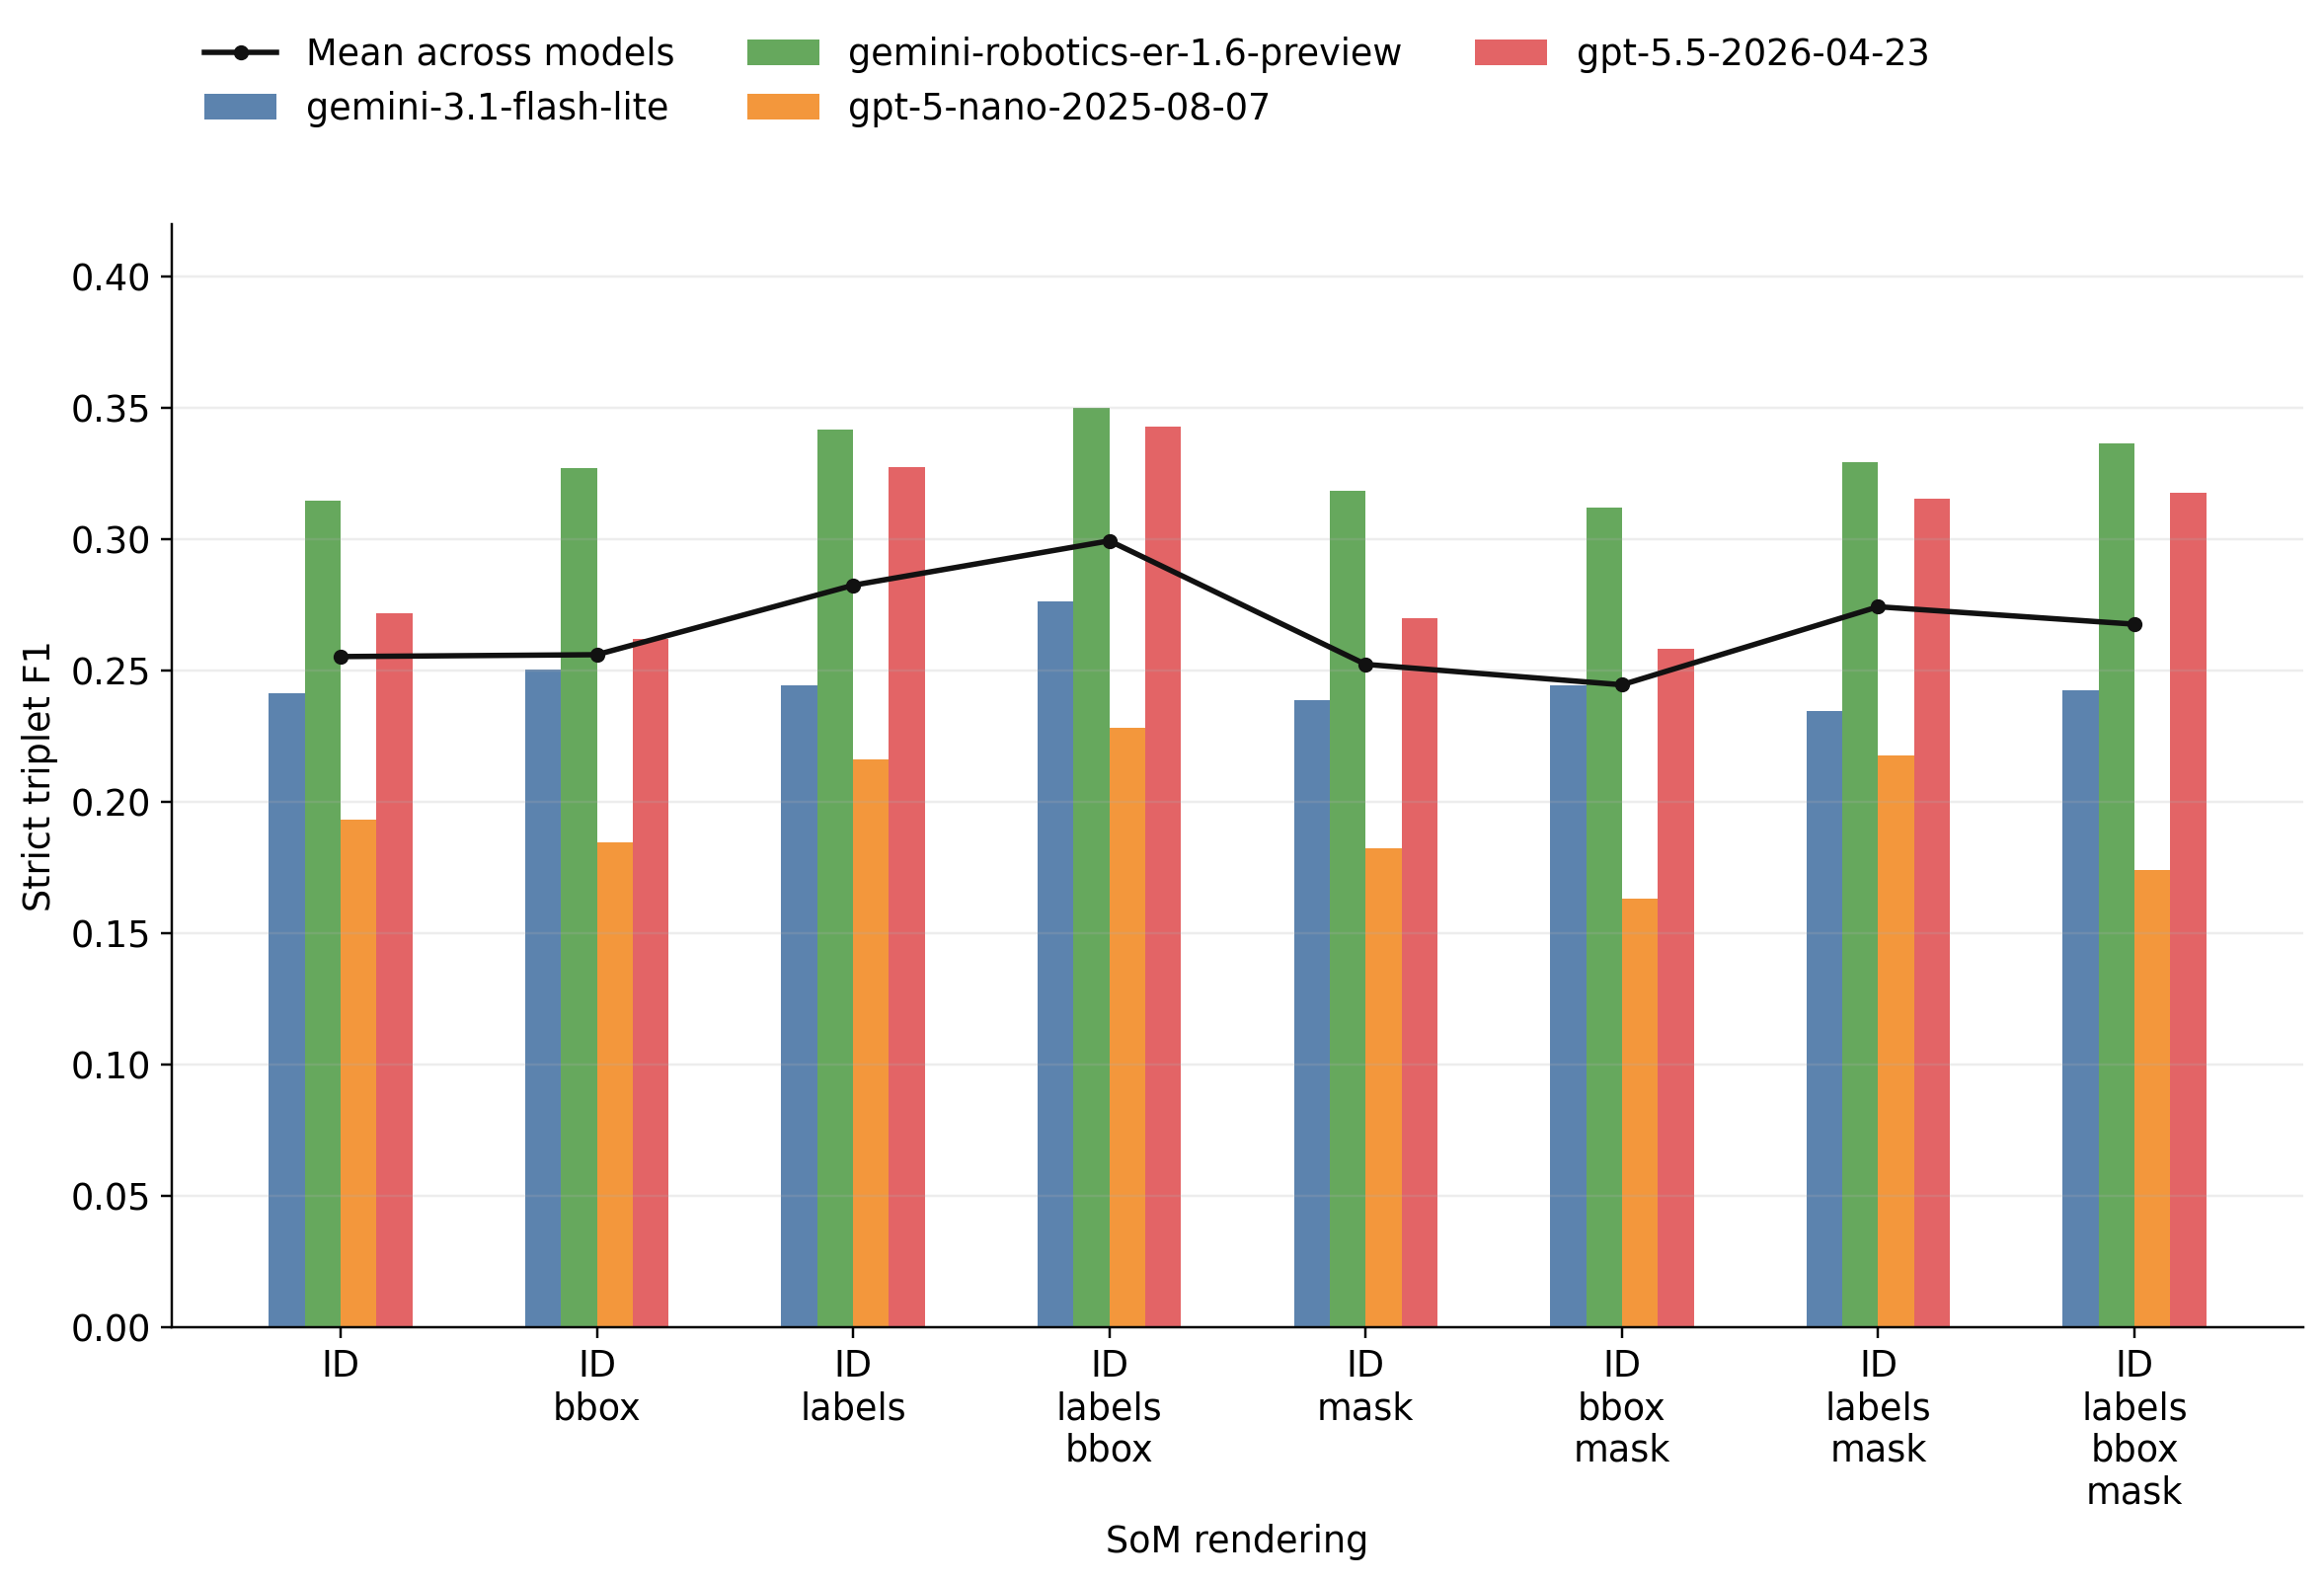
\includegraphics[width=\linewidth]{pics/best_som_strict_f1_grouped.pdf}
\caption{Strict triplet F1 for the evaluated SoM renderings. Each group corresponds to one visual prompting setting and each bar corresponds to one VLM family. The black line shows the mean across available models for the given setting.}\label{fig:best-som-strict-f1}
\end{figure}

\begin{table}[!htbp]
\centering
\small
\caption{Top SoM settings averaged across available model families. Settings are ordered by mean strict triplet F1.}\label{tab:best-som-settings}
\begin{tabular}{@{}lrrrr@{}}
\toprule
SoM setting & Strict & Attr. & Pair-O & Pair-U \\
\midrule
ID + labels + bbox & 0.301 & 0.390 & 0.405 & 0.538 \\
ID + labels & 0.283 & 0.366 & 0.399 & 0.551 \\
ID + labels + bbox + mask & 0.278 & 0.341 & 0.412 & 0.551 \\
\bottomrule
\end{tabular}
\end{table}

The aggregate results in Table~\ref{tab:best-som-settings} support the same conclusion. Class labels matter: variants with labels outperform variants that only show numeric IDs and boxes. Bounding boxes further improve strict triplet F1 by helping the model associate the label and ID with the correct visual region. Mask overlays do not consistently improve strict scene graph generation. They can slightly improve object-pair matching in some cases, but they also add visual clutter and tend to reduce exact relation or attribute correctness. It must be noted that we used, for computational reasons, GrabCut to generate masks, whereas the original SoM paper used SAM. For this reason, we use ID + class label + bounding box as the default SoM rendering in the following comparisons.

The next question was whether the selected SoM rendering actually helps compared with an unmarked raw image. This experiment used the two strongest VLM families from the previous ablation, Gemini Robotics and GPT-5.5. All conditions received the same frozen object detections and the same frozen vocabulary. The raw-image conditions received the original image, the object list, and the vocabulary. The SoM conditions received the marked image with IDs, labels, and bounding boxes, again together with the object list and vocabulary. Both variants were also tested with and without the generated scene description.

\begin{figure}[!htbp]
\centering
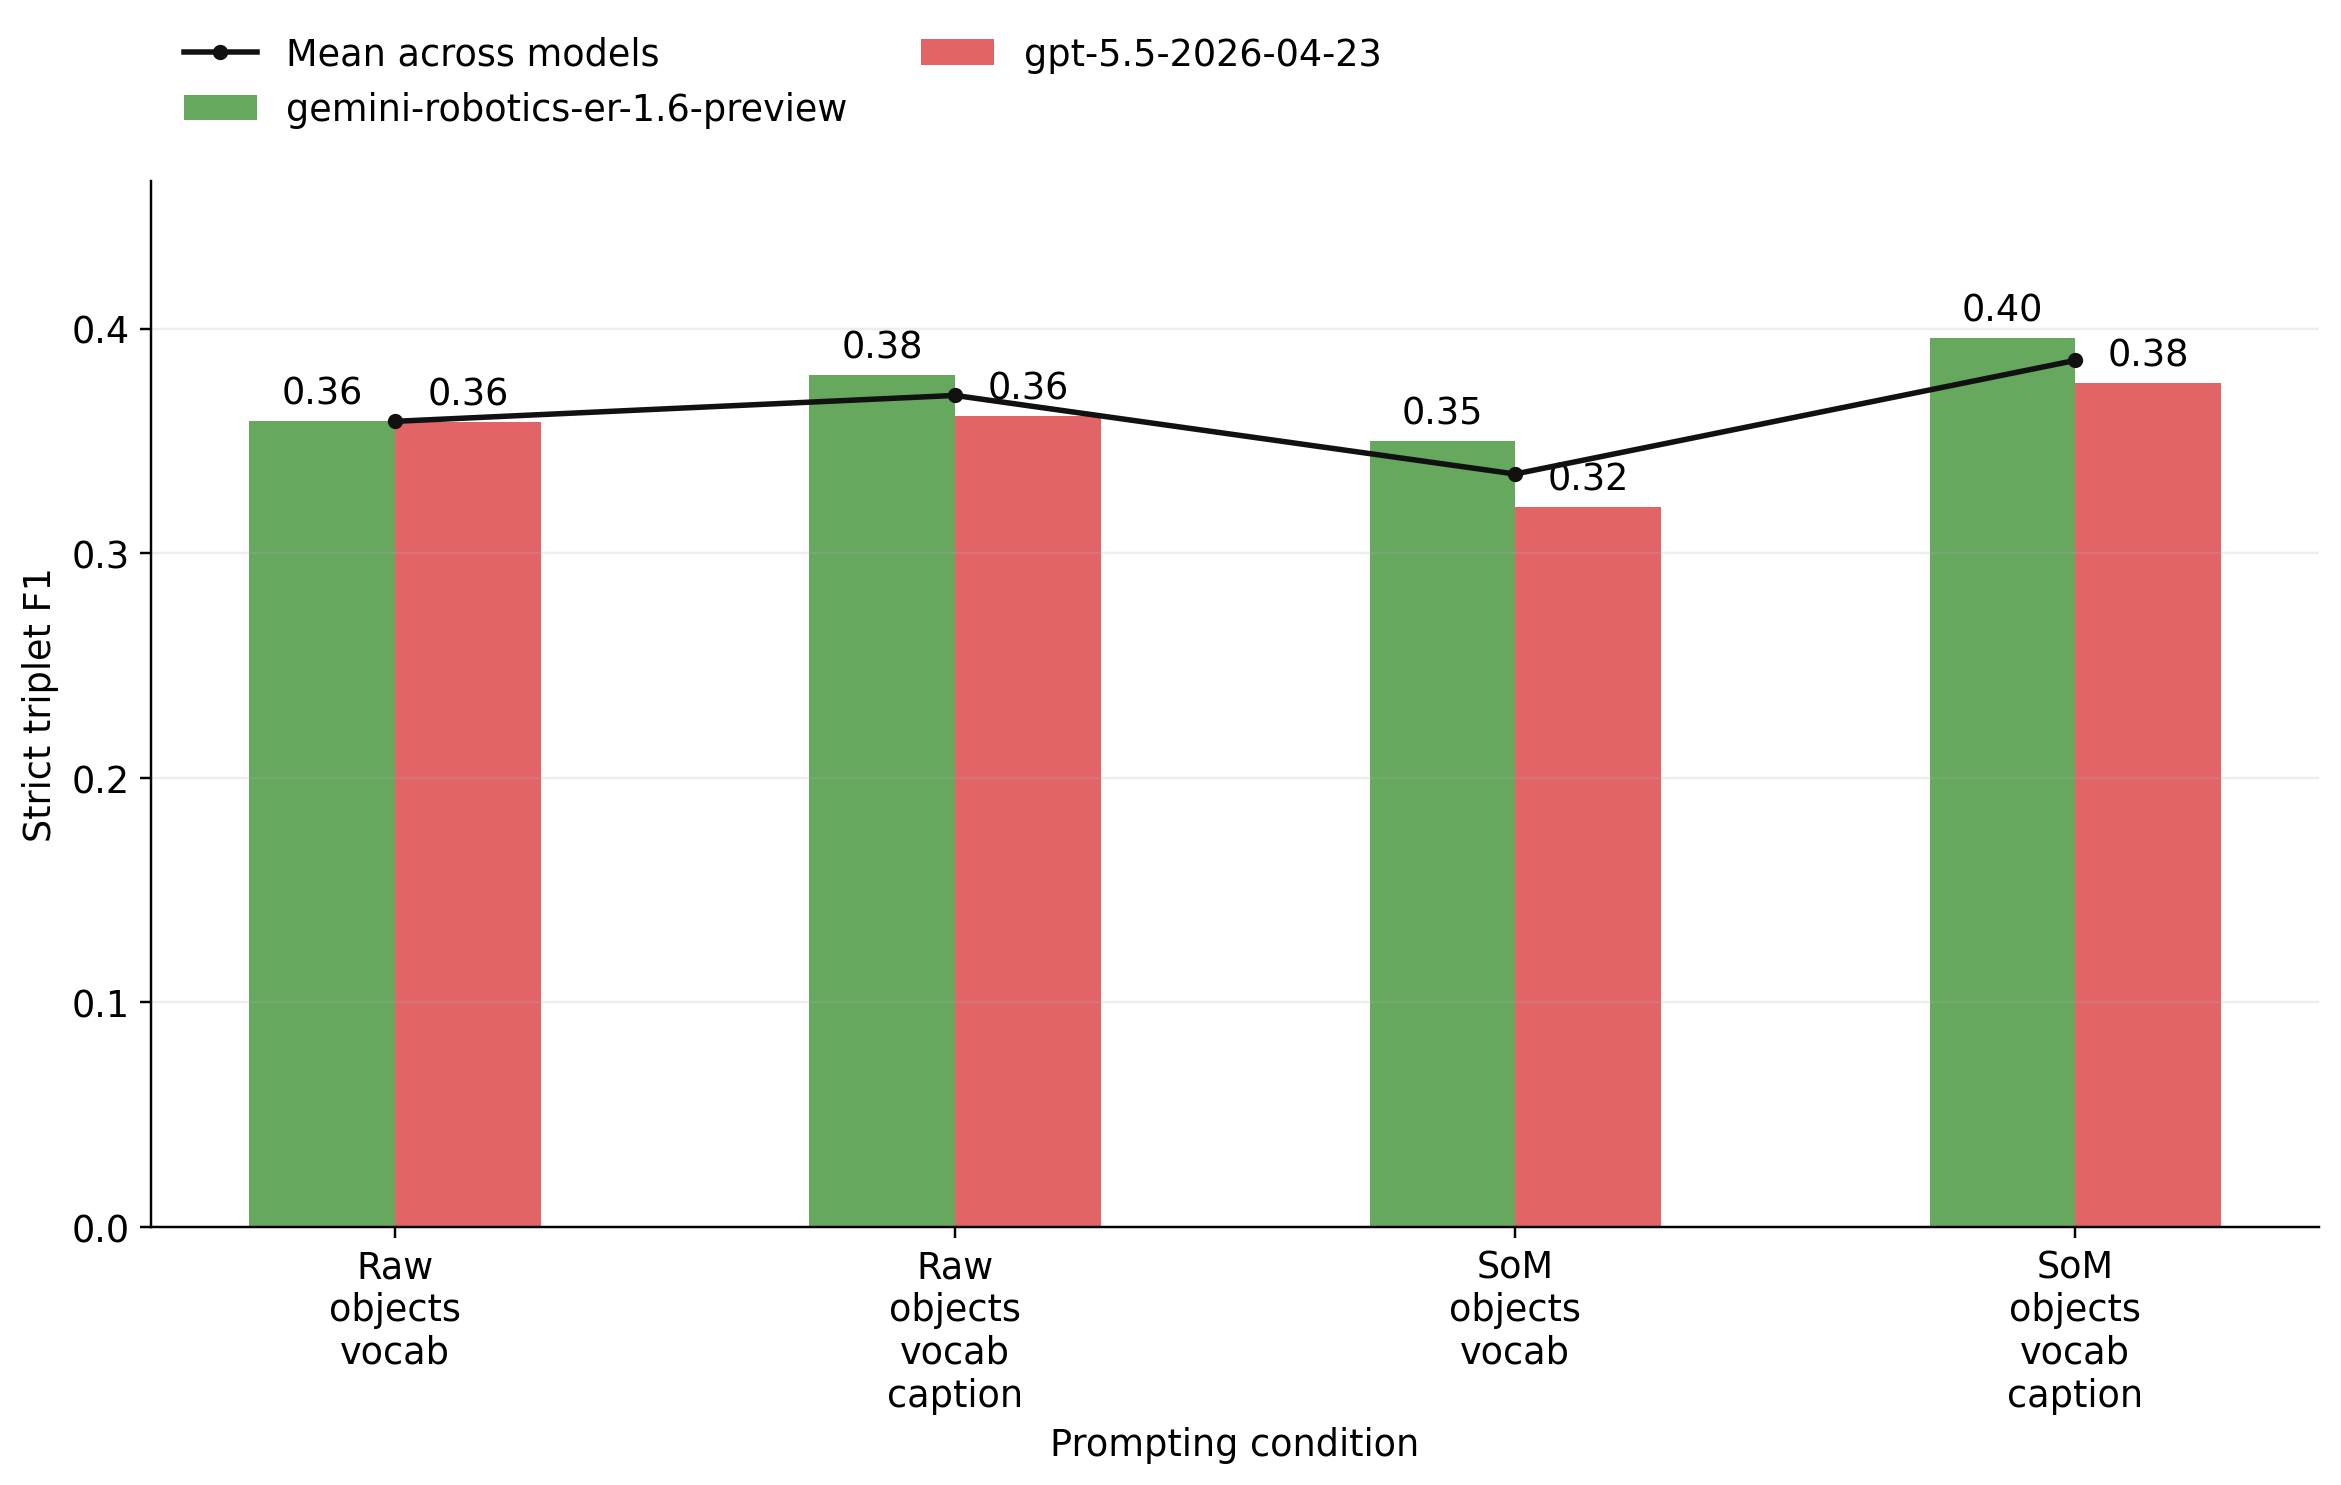
\includegraphics[width=\linewidth]{pics/som_vs_no_som_strict_f1_grouped.pdf}
\caption{Strict triplet F1 for raw-image and Set-of-Mark scene graph prompting. Both evaluated models perform best when SoM is combined with the object list, vocabulary, and scene description.}\label{fig:som-vs-no-som}
\end{figure}

\begin{table}[!htbp]
\centering
\scriptsize
\caption[Effect of SoM and scene descriptions.]{Effect of raw-image prompting, Set-of-Mark prompting, and scene descriptions on scene graph generation. All conditions include the frozen object list and vocabulary.}\label{tab:som-vs-no-som}
\begin{tabularx}{\linewidth}{@{}lXrrrr@{}}
\toprule
Model & Condition & Strict & Attr. & Pair-O & Pair-U \\
\midrule
Gemini Robotics & Raw & 0.359 & 0.447 & 0.515 & 0.664 \\
Gemini Robotics & Raw+caption & 0.379 & 0.507 & 0.482 & 0.663 \\
Gemini Robotics & SoM & 0.350 & 0.441 & 0.499 & 0.675 \\
Gemini Robotics & SoM+caption & \textbf{0.396} & \textbf{0.515} & \textbf{0.523} & \textbf{0.697} \\
GPT-5.5 & Raw & 0.358 & 0.407 & 0.510 & 0.663 \\
GPT-5.5 & Raw+caption & 0.361 & 0.426 & 0.516 & 0.656 \\
GPT-5.5 & SoM & 0.321 & 0.341 & 0.521 & 0.655 \\
GPT-5.5 & SoM+caption & \textbf{0.376} & \textbf{0.431} & \textbf{0.527} & \textbf{0.682} \\
\bottomrule
\end{tabularx}
\end{table}

Figure~\ref{fig:som-vs-no-som} and Table~\ref{tab:som-vs-no-som} show that SoM is most useful as a grounding layer, not as a replacement for semantic context. The raw image with an object list and vocabulary was already a strong baseline. Adding SoM without a caption slightly reduced strict F1 for Gemini Robotics, from 0.359 to 0.350, and more clearly for GPT-5.5, from 0.358 to 0.321. Once the scene description was included, however, the marked image produced the best result for both models. Gemini Robotics improved from 0.379 to 0.396, and GPT-5.5 improved from 0.361 to 0.376. The caption supplies scene-level semantics; SoM anchors those semantics to detector IDs and visible object regions.

This interpretation also fits the evaluation set and the real Pepper deployment. Many images are low-resolution, blurred, or visually dense. In those cases, labels and boxes can become clutter if the marked image is the only source of scene semantics. This eems to hint on the fact that in such cases the textual information on the image content helps the model when it can't see it itself. The per-image results show the same tension. On a cleaner office image, SoM without a caption improved strict F1 for both models: Gemini Robotics rose from 0.320 to 0.467, and GPT-5.5 from 0.333 to 0.400. On a cluttered living-room image, SoM alone reduced performance, but SoM with a caption outperformed the raw image with a caption for both models: Gemini Robotics improved from 0.513 to 0.653, and GPT-5.5 from 0.464 to 0.500. SoM is therefore useful for object-ID grounding, but it is most reliable when paired with a textual scene description.

The gap between pair metrics and strict triplet F1 is also informative. In the SoM-design ablation, the best runs reached unordered pair F1 around 0.59--0.61 while strict triplet F1 remained around 0.35. In the SoM-versus-raw prompting experiment, the best condition increased unordered pair F1 to 0.697 and strict triplet F1 to 0.396. The pattern is consistent: the models often detect that two objects should be related, but still fail on the exact predicate, relation direction, or attribute assignment. For dialogue, that distinction matters. Knowing that two objects are related may be enough for some follow-up questions, but exact spatial or attribute questions require the stricter graph representation.

We also examined whether the generated scene graphs were too dense or too sparse compared with the human annotations. This was computed over the SoM-design experiment by comparing each generated graph to the same human-labeled graph. The absolute label counts are therefore aggregated over repeated model runs; the ratios matter more. The main pattern is that the models do not simply overgenerate or undergenerate all graph edges uniformly. Instead, they tend to overgenerate unary attributes and undergenerate binary relations. For example, the Gemini Robotics ID+label+bbox run produced only 0.80 times as many total edges as the human annotation, but 1.59 times as many attributes and only 0.46 times as many binary relations. GPT-5.5 was denser overall, with 1.12 times as many total edges, but still showed the same shift toward attributes: 1.90 times as many attributes and 0.79 times as many binary relations.

\begin{table}[!htbp]
\centering
\scriptsize
\caption{Generation density for representative SoM-design runs. Ratios compare the number of generated edges to the number of human-annotated edges.}\label{tab:generation-density}
\begin{tabular}{@{}lrrrrrr@{}}
\toprule
Run & Edge & Attr. & Rel. & Prec. & Rec. & F1 \\
\midrule
Gemini Flash, ID+labels+bbox & 0.55 & 0.87 & 0.42 & 0.39 & 0.21 & 0.27 \\
Gemini Robotics, ID+labels+bbox & 0.80 & 1.59 & 0.46 & 0.44 & 0.35 & 0.39 \\
Gemini Pro, ID+labels+bbox & 0.91 & 1.38 & 0.71 & 0.36 & 0.33 & 0.34 \\
GPT nano, ID+labels+bbox & 0.54 & 0.92 & 0.37 & 0.36 & 0.20 & 0.25 \\
GPT-5.5, ID+labels+bbox & 1.12 & 1.90 & 0.79 & 0.36 & 0.40 & 0.38 \\
\bottomrule
\end{tabular}
\end{table}

The label-level analysis gives a more concrete explanation of this behavior and mirrors the long-tail difficulty discussed in Section~\ref{sec:grounding-sgg}. Among binary relations, broad spatial predicates were most often missed. The relation \texttt{next\_to} was generated at only 0.28 times its human-annotated frequency, \texttt{right\_of} at 0.42, \texttt{above} at 0.40, \texttt{below} at 0.27, and \texttt{supporting} at 0.14. In contrast, \texttt{in\_front\_of} and \texttt{sitting\_on} were overgenerated, at 1.18 and 1.97 times their annotated frequency respectively. The best classified relations were visually concrete or action-like. The strongest was \texttt{holding} (F1 0.80), followed by \texttt{lying\_on} (0.63) and \texttt{working\_on} (0.59). The common spatial predicate \texttt{on} was also comparatively reliable, with F1 0.49 and a generation ratio close to one.

\begin{table}[!htbp]
\centering
\scriptsize
\caption{Selected label-level generation patterns aggregated over the SoM-design experiment.}\label{tab:label-generation-patterns}
\begin{tabular}{llrrrr}
\toprule
Type & Label & Pred./GT ratio & Precision & Recall & F1 \\
\midrule
Over-generated relation & \texttt{in\_front\_of} & 1.18 & 0.09 & 0.10 & 0.09 \\
Over-generated relation & \texttt{sitting\_on} & 1.97 & 0.30 & 0.59 & 0.40 \\
Under-generated relation & \texttt{next\_to} & 0.28 & 0.35 & 0.10 & 0.16 \\
Under-generated relation & \texttt{supporting} & 0.14 & 0.56 & 0.08 & 0.13 \\
Best relation & \texttt{holding} & 0.86 & 0.87 & 0.74 & 0.80 \\
Best relation & \texttt{lying\_on} & 0.71 & 0.76 & 0.54 & 0.63 \\
\midrule
Over-generated attribute & \texttt{rectangular} & 7.28 & 0.08 & 0.61 & 0.15 \\
Over-generated attribute & \texttt{large} & 5.00 & 0.07 & 0.35 & 0.12 \\
Under-generated attribute & \texttt{plastic} & 0.31 & 0.31 & 0.10 & 0.15 \\
Under-generated attribute & \texttt{yellow} & 0.43 & 0.50 & 0.22 & 0.30 \\
Best attribute & \texttt{red} & 0.89 & 0.82 & 0.73 & 0.77 \\
Best attribute & \texttt{black} & 1.25 & 0.47 & 0.59 & 0.52 \\
\bottomrule
\end{tabular}
\end{table}

For attributes, the opposite error profile appears. The models often assign visually plausible attributes too broadly. Shape and size terms are especially affected: \texttt{rectangular} was generated 7.28 times more often than in the human annotations and \texttt{large} 5.00 times more often, but both had low precision. Color attributes were easier. The best attribute was \texttt{red}, with F1 0.77, followed by common attributes such as \texttt{black}, \texttt{standing}, \texttt{green}, \texttt{gray}, and \texttt{wooden}. This supports the interpretation that VLMs are relatively strong at assigning salient appearance attributes, but weaker at producing complete and correctly directed relational graphs.

The ground truth annotations were produced by manually correcting drafted scene graphs. This makes annotation faster and keeps the labels aligned with the detector IDs, but it can also anchor the final labels to the style of the initial drafts. The ranking should therefore be read cautiously. The more robust conclusion is the visualization result: across the evaluated VLMs, object IDs combined with class labels and bounding boxes provide the strongest and most stable SoM representation for ID-grounded scene graph generation.

\section{Vocabulary Size Sensitivity}

The previous experiments used the full frozen vocabulary of 50 predicates and 25 attributes. While this maximizes the expressive space available to the model, it also increases prompt length and token cost, and may make predicate selection less reliable by introducing more semantically similar alternatives. We therefore ran a vocabulary-size sensitivity experiment to test whether scene-graph quality depends mainly on the number of available labels or also on how those labels are compressed.

All runs used the same evaluation split, the same frozen detections, the same SoM setting with IDs, class labels, and bounding boxes, and the same Gemini Robotics model. The prompt used a flat shuffled vocabulary list, so predicates and attributes were not separated. For each vocabulary level, both the generated scene graph and the ground truth were mapped into the reduced vocabulary before evaluation. If \texttt{sitting\_on} was mapped to \texttt{on}, for example, then both prediction and ground truth were evaluated with the reduced label \texttt{on}. The experiment therefore measures whether a smaller controlled vocabulary preserves enough task-relevant information, not whether the model can predict labels that were removed from the prompt.

We compared three reduction strategies. The semantic strategy was manually designed by grouping related concepts, for example mapping \texttt{sitting\_on}, \texttt{standing\_on}, \texttt{lying\_on}, and \texttt{resting\_on} to \texttt{on}, or mapping many appearance attributes to coarser labels such as \texttt{colored}, \texttt{sized}, \texttt{shaped}, and \texttt{textured}. The frequency strategy kept the most frequent labels in the human-labeled evaluation graphs and mapped removed labels to retained labels from a related group when possible. The random strategy used the same vocabulary sizes but selected and mapped labels randomly with a fixed seed. This random baseline separates the effect of having fewer labels from the effect of choosing a meaningful reduced vocabulary.

\begin{figure}[!htbp]
\centering
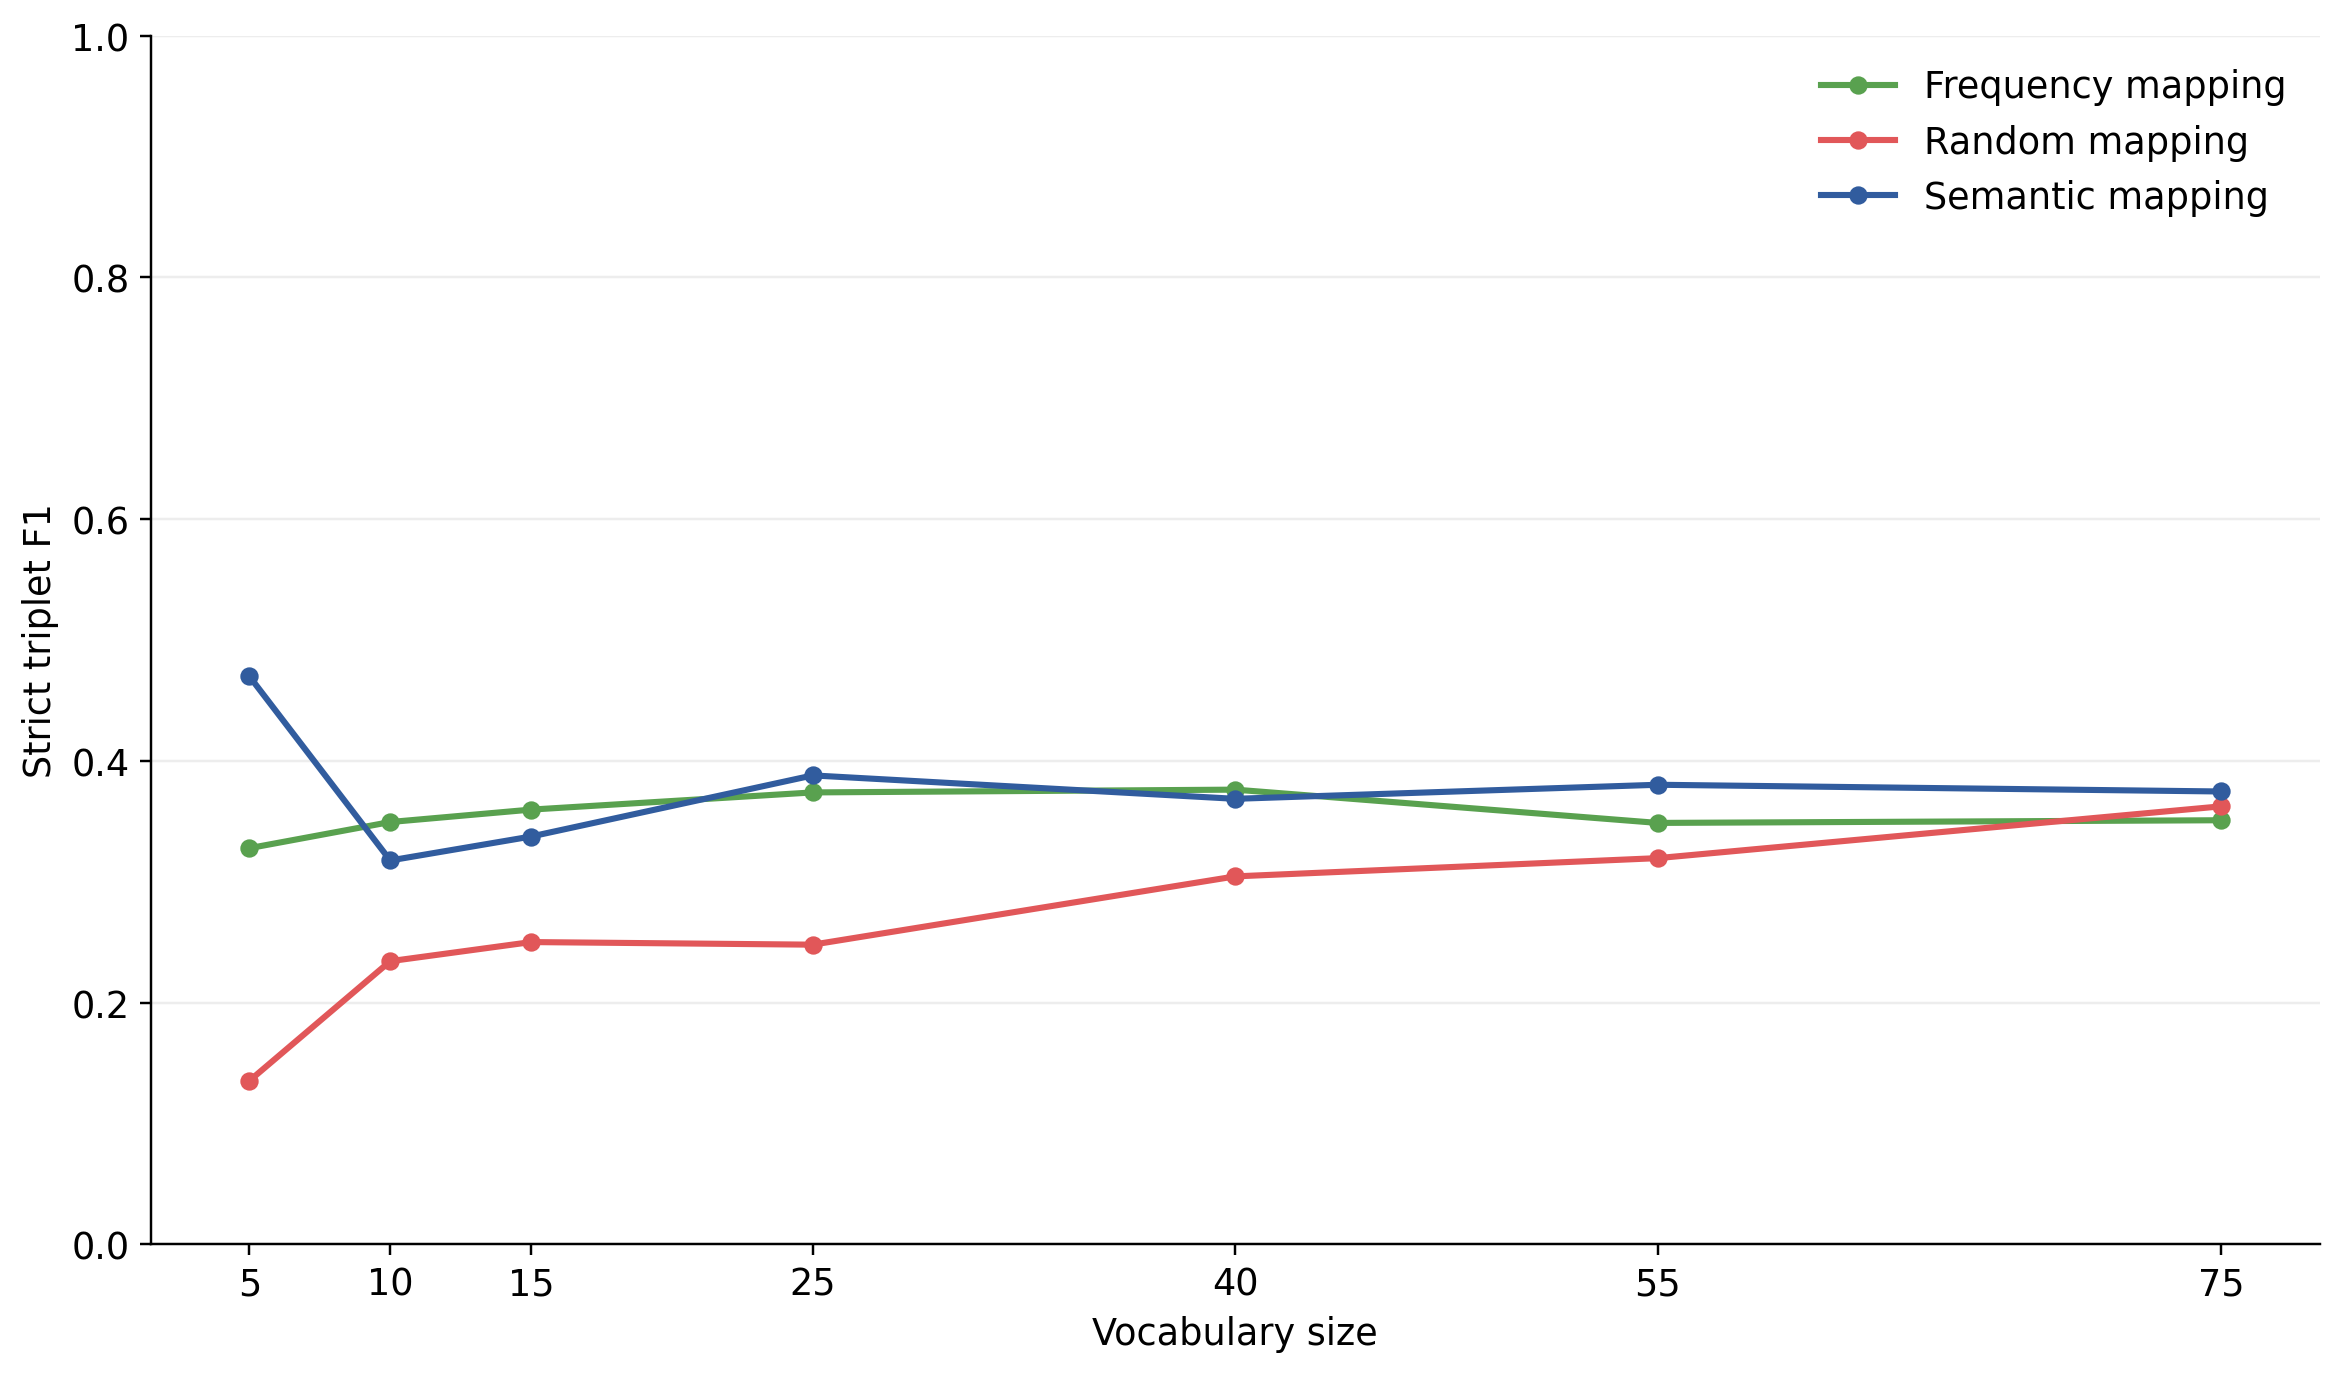
\includegraphics[width=\linewidth]{pics/context_rot_strict_f1_compare.pdf}
\caption{Strict triplet F1 under different vocabulary-size reductions. Semantic and frequency-based reductions preserve performance much better than random reductions, showing that vocabulary constitution matters, not only vocabulary size.}\label{fig:context-rot-strict}
\end{figure}

\begin{table}[!htbp]
\centering
\small
\caption{Selected strict triplet F1 values from the vocabulary-size sensitivity experiment.}\label{tab:context-rot-strict}
\begin{tabular}{lrrrr}
\toprule
Reduction strategy & 5 terms & 15 terms & 25 terms & 75 terms \\
\midrule
Semantic mapping & \textbf{0.470} & 0.337 & \textbf{0.388} & \textbf{0.375} \\
Frequency mapping & 0.328 & \textbf{0.360} & 0.374 & 0.351 \\
Random mapping & 0.135 & 0.250 & 0.248 & 0.362 \\
\bottomrule
\end{tabular}
\end{table}

The results in Figure~\ref{fig:context-rot-strict} and Table~\ref{tab:context-rot-strict} show that vocabulary constitution has a clear effect. Random reductions underperform the semantic and frequency-based reductions at every reduced vocabulary size. That is expected: random compression can remove central spatial labels and map semantically different relations to arbitrary labels. The model receives a shorter prompt, but the remaining labels are less coherent for the task.

The semantic and frequency strategies are much closer to each other. That is also expected, because the most frequent terms in this domain are already semantically central: \texttt{next\_to}, \texttt{left\_of}, \texttt{right\_of}, \texttt{above}, \texttt{below}, and \texttt{on} for predicates, and common color and material attributes for unary labels. The difference is largest at the smallest vocabularies. With only five terms, the semantic mapping reaches strict F1 of 0.470, while the frequency mapping reaches 0.328. This does not mean that a five-term vocabulary is sufficient for the final system. It means that an extremely coarse semantic mapping can inflate strict F1 by collapsing many distinctions into a few broad labels such as \texttt{next\_to}, \texttt{on}, \texttt{touching}, and \texttt{visible}. The task becomes easier because many originally different annotations become equivalent after mapping.

The more useful region is the middle of the curve. At 15--25 terms, the semantic and frequency reductions already approach or exceed the full-vocabulary strict F1. The semantic 25-term vocabulary reached 0.388, compared with 0.375 for the full 75-term vocabulary. The frequency vocabulary reached 0.360 with 15 terms and 0.374 with 25 terms. Adding more terms after this point did not produce a clear improvement. This suggests that most of the dialogue-relevant scene-graph information in this dataset is carried by a small core vocabulary. Larger vocabularies add expressivity, but they also add more possible near-miss labels and more prompt tokens.

The compact vocabularies also make this interpretation intuitive. The semantic 15-term level keeps the predicates \texttt{above}, \texttt{below}, \texttt{left\_of}, \texttt{right\_of}, \texttt{next\_to}, \texttt{in}, \texttt{on}, \texttt{using}, and \texttt{touching}, plus coarse attributes for color, transparency, openness, size, shape, and texture. The frequency 15-term level keeps mostly the same spatial core, but preserves concrete frequent attributes such as \texttt{black}, \texttt{white}, \texttt{wooden}, \texttt{green}, \texttt{red}, and \texttt{gray}. In both cases, the reduced vocabulary still preserves the main relations that matter for office and robot-dialogue scenes. The random vocabulary lacks this structure, which explains its weaker performance.

We therefore interpret vocabulary reduction as a useful design tool rather than only an ablation. A compact vocabulary of roughly 15--25 well-chosen concepts appears to be enough for much of the evaluated scene-graph task, while being cheaper to prompt with and easier to control. The full vocabulary remains useful when more detailed dialogue is required, but the sensitivity experiment shows that simply adding more labels is not always beneficial under strict graph metrics.

\section{Vocabulary Presentation Format}

Finally, we tested whether the format in which the vocabulary is presented to the VLM affects scene-graph generation. All runs used the same evaluation split, frozen detections, full frozen vocabulary, SoM image with IDs, class labels, and bounding boxes, object list, and scene description. The only changed variable was the vocabulary rendering in the prompt. In the list condition, predicates and attributes were merged into one flat shuffled list. In the dictionary condition, the same terms were presented as a structured object with separate predicate and attribute lists.

\begin{table}[!htbp]
\centering
\scriptsize
\caption{Effect of vocabulary presentation format. The list format presents predicates and attributes as one shuffled flat list; the dictionary format separates predicates from attributes.}\label{tab:vocab-presentation}
\begin{tabular}{llrrrr}
\toprule
Model & Format & Strict F1 & Attr. F1 & Pair ord. F1 & Pair unord. F1 \\
\midrule
Gemini Flash & List & 0.331 & 0.470 & 0.491 & 0.678 \\
Gemini Flash & Dictionary & \textbf{0.367} & \textbf{0.503} & 0.489 & \textbf{0.688} \\
Gemini Robotics & List & 0.396 & 0.483 & \textbf{0.534} & 0.695 \\
Gemini Robotics & Dictionary & \textbf{0.412} & \textbf{0.526} & 0.521 & \textbf{0.714} \\
GPT nano & List & \textbf{0.313} & \textbf{0.472} & \textbf{0.356} & \textbf{0.537} \\
GPT nano & Dictionary & 0.262 & 0.414 & 0.318 & 0.488 \\
GPT-5.5 & List & \textbf{0.378} & \textbf{0.447} & 0.519 & \textbf{0.675} \\
GPT-5.5 & Dictionary & 0.361 & 0.423 & \textbf{0.522} & 0.666 \\
\bottomrule
\end{tabular}
\end{table}

The result is not a universal win for either representation. The two Gemini-family models performed better with the dictionary presentation. Gemini Flash improved from strict F1 0.331 to 0.367, and Gemini Robotics improved from 0.396 to 0.412. The attribute metric improved in both cases, which suggests that explicitly separating predicates from attributes may help these models avoid some label-role confusion. In contrast, the GPT-family models performed better with the flat list. GPT nano improved from 0.262 to 0.313 strict F1 when using the list, and GPT-5.5 improved from 0.361 to 0.378. For GPT-5.5, the ordered pair metric was almost unchanged, which suggests that the main difference was not object pairing but exact label selection.

We therefore treat this experiment as inconclusive at the system level, but informative for prompt design. Vocabulary presentation is a model-dependent prompt detail. The safer conclusion is that vocabulary constitution and visual grounding matter more than the exact list-versus-dictionary formatting. However, when optimizing for a specific model family, the formatting should be treated as a small but measurable hyperparameter. In our experiments, structured dictionary presentation was preferable for Gemini models, while a flat shuffled list was preferable for GPT models.

\section{Dialogue and Interaction Results}

Besides offline evaluation, we also measured the latency of the complete robot interaction loop. We report the time to first spoken answer, which is analogous to time-to-first-token in text generation systems, but measured at the robot interaction level. This value includes ASR and dialogue dispatch, robot-side method scheduling, image transfer, server processing, network communication, and TTS startup. The measurement combines two sources. First, we logged the client-side time from the accepted QiChat turn to the moment when the final answer was sent to the robot speech system. Second, we measured several complete interactions manually with a phone stopwatch, because that better captures the perceived delay from the user's point of view. When two manual values are reported, the first value denotes the moment when the robot started an acknowledgement or introductory sentence, and the second value denotes the moment when the substantive answer started.

\begin{table}[!htbp]
\centering
\caption[Robot-side latency by turn type.]{Robot-side latency by turn type, in seconds. Answer time is measured from the accepted dialogue turn to the start of final answer speech. Server and pre-server columns split that interval around the client request.}\label{tab:robot-latency}
\scriptsize
\begin{tabular}{@{}lrrrrr@{}}
\toprule
Operation & $n$ & Med. ans. & Mean ans. & Med. srv. & Med. pre. \\
\midrule
Look / describe scene & 18 & 11.36 & 11.63 $\pm$ 2.47 & 3.47 & 7.49 \\
Ask question & 7 & 4.33 & 4.75 $\pm$ 1.34 & 1.12 & 3.52 \\
Cached answer & 1 & 0.009 & 0.009 & -- & -- \\
\bottomrule
\end{tabular}
\end{table}

The latency profile separates visual perception from memory-based dialogue. Follow-up questions over existing memory were answered with a median latency of 4.33 seconds, which is acceptable for spoken human--robot interaction when the robot gives short acknowledgement feedback. Visual description turns were slower, with a median latency of 11.36 seconds. Only 3.47 seconds of that median interval was spent waiting for the server response; the larger part, 7.49 seconds, happened before the client issued the server request.

This pre-server delay has several sources. Part of it comes from the robot-side interaction pipeline, image acquisition, and the placement of some acknowledgement utterances in QiChat before the bound Python method starts executing. In such cases, the robot speaks an introductory sentence before the method has started, so perception cannot run concurrently with the acknowledgement. That is useful from the user's perspective because it removes silence while the robot appears to be processing the request, but it also means that some computation starts later than necessary. Moving such acknowledgements into the client method, or starting the method before longer introductory speech, would allow perception to run while the robot is already speaking.

Another source of latency is the distributed deployment itself. In the real robot setup, the image must be captured on Pepper, sent to the server, processed locally and/or by cloud VLM services, and the resulting answer must then be returned to the robot. Therefore, the measured latency includes not only model inference, but also network transfer and communication overhead between Pepper, the local server, and external cloud services. This is especially visible for VLM-based scene-graph construction, where the image and prompt may leave the robot-server loop and go through a cloud model before the answer returns.

For comparison, we also ran the same kind of visual processing with a virtual robot in Choregraphe, where the image was already available on the server machine and did not have to be captured and transmitted from Pepper. In two such runs, the backend wall-processing time was 7.47 seconds and 3.98 seconds. The corresponding scene-graph generation times were 4.49 seconds and 2.38 seconds. These values are lower than the slower real-robot interaction cases and indicate that robot capture, transfer, cloud communication, and turn orchestration contribute substantially to the end-to-end latency.

We also tested several backend configurations manually. The local LLM setup used a small Qwen3.5-0.8B GGUF model from Unsloth,\footnote{\url{https://huggingface.co/unsloth/Qwen3.5-0.8B-GGUF}} served through llama.cpp on an NVIDIA RTX 5050 with 8 GB VRAM. The same GPU also hosted detection, embedding computation, and other visual components, so the setup represents a constrained local deployment rather than an isolated benchmark. In this configuration, normal question answering was still usable for dialogue. The expensive operations were not short chat answers, but VLM-based scene-graph generation and pregeneration of suggested questions.

This distinction is important for deployment. Pregenerated questions are useful because cached answers are effectively immediate: in the logged run, the cached answer latency was 0.009 seconds. However, the pregeneration itself does not have to be part of the interactive robot--server loop. It can be run offline, scheduled after perception, or replaced by administrator-authored questions uploaded to the robot. This keeps the benefit of immediate answers without forcing the user to wait for question generation.

The fastest measured backend configuration was the rule/RELTR-based scene-graph path without VLM scene-graph generation. In the manual notes this setup had server wall-processing times below one second, with scene-graph generation around a tenth of a second. This shows that the system can be responsive when the expensive VLM reasoning path is disabled. The VLM path is more expressive and useful for richer memory construction, but it should be treated as an optional or asynchronous memory-building process rather than a blocking step for every spoken response.

Overall, these measurements suggest that the architecture is practical for memory-based dialogue. Once the scene memory exists, follow-up questions can be answered within a few seconds, and cached answers are immediate. The remaining latency problem is mainly in visual memory construction, cloud and network communication, and in the ordering of robot acknowledgements relative to method execution. Therefore, the practical deployment strategy is to answer from existing memory whenever possible, use cached or curated questions for common interactions, and run expensive scene-graph updates outside the critical response path.

% \section{Architectural Discussion}
% \begin{itemize}
%     \item Reflect on the main architectural choices:
%     \begin{itemize}
%         \item remote inference versus onboard intelligence;
%         \item in-process versus worker runtime;
%         \item explicit scene memory versus implicit conversational context;
%         \item hybrid graph generation versus a single-model solution.
%     \end{itemize}
%     \item Explain what worked well and what remains engineering debt.
% \end{itemize}

% \section{Limitations}
% \begin{itemize}
%     \item Current reliance on external compute and network connectivity.
%     \item Limited long-term memory and lack of a richer knowledge layer beyond current scene state and short conversation history.
%     \item Dependence on prompt quality and provider reliability.
%     \item Incomplete evaluation of some exploratory training paths if they remain unfinished.
%     \item Potential mismatch between offline graph metrics and perceived dialogue quality in real HRI.
% \end{itemize}
